%%%%%%%%%%%%%%%%%%%%%%%%%%%%%%%%%%%%%%%%%
% Programming/Coding Assignment
% LaTeX Template
%
% This template has been downloaded from:
% http://www.latextemplates.com
%
% Original author:
% Ted Pavlic (http://www.tedpavlic.com)
%
% Note:
% The \lipsum[#] commands throughout this template generate dummy text
% to fill the template out. These commands should all be removed when 
% writing assignment content.
%
% This template uses a Perl script as an example snippet of code, most other
% languages are also usable. Configure them in the "CODE INCLUSION 
% CONFIGURATION" section.
%
%%%%%%%%%%%%%%%%%%%%%%%%%%%%%%%%%%%%%%%%%

%----------------------------------------------------------------------------------------
%	PACKAGES AND OTHER DOCUMENT CONFIGURATIONS
%----------------------------------------------------------------------------------------

\documentclass{article}

\usepackage{fancyhdr} % Required for custom headers
\usepackage{lastpage} % Required to determine the last page for the footer
\usepackage{extramarks} % Required for headers and footers
\usepackage[usenames,dvipsnames]{color} % Required for custom colors
\usepackage{graphicx} % Required to insert images
\usepackage{listings} % Required for insertion of code
\usepackage{courier} % Required for the courier font
\usepackage{hyperref} % Used for Hyper Linking
\usepackage{amsmath} % Used for Math


% Margins
\topmargin=-0.45in
\evensidemargin=0in
\oddsidemargin=0in
\textwidth=6.5in
\textheight=9.0in
\headsep=0.25in

\linespread{1.1} % Line spacing

% Set up the header and footer
\pagestyle{fancy}
\lhead{\hmwkAuthorName} % Top left header
\chead{\hmwkClass\ (\hmwkClassInstructor): \hmwkTitle} % Top center head
\rhead{\firstxmark} % Top right header
\lfoot{\lastxmark} % Bottom left footer
\cfoot{} % Bottom center footer
\rfoot{Page\ \thepage\ of\ \protect\pageref{LastPage}} % Bottom right footer
\renewcommand\headrulewidth{0.4pt} % Size of the header rule
\renewcommand\footrulewidth{0.4pt} % Size of the footer rule

\setlength\parindent{0pt} % Removes all indentation from paragraphs

%----------------------------------------------------------------------------------------
%	CODE INCLUSION CONFIGURATION
%----------------------------------------------------------------------------------------

\definecolor{MyDarkGreen}{rgb}{0.0,0.4,0.0} % This is the color used for comments
\lstloadlanguages{Perl} % Load Perl syntax for listings, for a list of other languages supported see: ftp://ftp.tex.ac.uk/tex-archive/macros/latex/contrib/listings/listings.pdf
\lstset{language=Perl, % Use Perl in this example
        frame=single, % Single frame around code
        basicstyle=\small\ttfamily, % Use small true type font
        keywordstyle=[1]\color{Blue}\bf, % Perl functions bold and blue
        keywordstyle=[2]\color{Purple}, % Perl function arguments purple
        keywordstyle=[3]\color{Blue}\underbar, % Custom functions underlined and blue
        identifierstyle=, % Nothing special about identifiers                                         
        commentstyle=\usefont{T1}{pcr}{m}{sl}\color{MyDarkGreen}\small, % Comments small dark green courier font
        stringstyle=\color{Purple}, % Strings are purple
        showstringspaces=false, % Don't put marks in string spaces
        tabsize=5, % 5 spaces per tab
        %
        % Put standard Perl functions not included in the default language here
        morekeywords={rand},
        %
        % Put Perl function parameters here
        morekeywords=[2]{on, off, interp},
        %
        % Put user defined functions here
        morekeywords=[3]{test},
       	%
        morecomment=[l][\color{Blue}]{...}, % Line continuation (...) like blue comment
        numbers=left, % Line numbers on left
        firstnumber=1, % Line numbers start with line 1
        numberstyle=\tiny\color{Blue}, % Line numbers are blue and small
        stepnumber=5 % Line numbers go in steps of 5
}

% Creates a new command to include a perl script, the first parameter is the filename of the script (without .pl), the second parameter is the caption
\newcommand{\perlscript}[2]{
\begin{itemize}
\item[]\lstinputlisting[caption=#2,label=#1]{#1.pl}
\end{itemize}
}

%----------------------------------------------------------------------------------------
%	DOCUMENT STRUCTURE COMMANDS
%	Skip this unless you know what you're doing
%----------------------------------------------------------------------------------------

% Header and footer for when a page split occurs within a problem environment
\newcommand{\enterProblemHeader}[1]{
\nobreak\extramarks{#1}{#1 continued on next page\ldots}\nobreak
\nobreak\extramarks{#1 (continued)}{#1 continued on next page\ldots}\nobreak
}

% Header and footer for when a page split occurs between problem environments
\newcommand{\exitProblemHeader}[1]{
\nobreak\extramarks{#1 (continued)}{#1 continued on next page\ldots}\nobreak
\nobreak\extramarks{#1}{}\nobreak
}

\setcounter{secnumdepth}{0} % Removes default section numbers
\newcounter{homeworkProblemCounter} % Creates a counter to keep track of the number of problems

\newcommand{\homeworkProblemName}{}
\newenvironment{homeworkProblem}[1][Problem \arabic{homeworkProblemCounter}]{ % Makes a new environment called homeworkProblem which takes 1 argument (custom name) but the default is "Problem #"
\stepcounter{homeworkProblemCounter} % Increase counter for number of problems
\renewcommand{\homeworkProblemName}{#1} % Assign \homeworkProblemName the name of the problem
\section{\homeworkProblemName} % Make a section in the document with the custom problem count
\enterProblemHeader{\homeworkProblemName} % Header and footer within the environment
}{
\exitProblemHeader{\homeworkProblemName} % Header and footer after the environment
}

\newcommand{\problemAnswer}[1]{ % Defines the problem answer command with the content as the only argument
\noindent\framebox[\columnwidth][c]{\begin{minipage}{0.98\columnwidth}#1\end{minipage}} % Makes the box around the problem answer and puts the content inside
}

\newcommand{\homeworkSectionName}{}
\newenvironment{homeworkSection}[1]{ % New environment for sections within homework problems, takes 1 argument - the name of the section
\renewcommand{\homeworkSectionName}{#1} % Assign \homeworkSectionName to the name of the section from the environment argument
\subsection{\homeworkSectionName} % Make a subsection with the custom name of the subsection
\enterProblemHeader{\homeworkProblemName\ [\homeworkSectionName]} % Header and footer within the environment
}{
\enterProblemHeader{\homeworkProblemName} % Header and footer after the environment
}

%----------------------------------------------------------------------------------------
%	HYPERLINK CUSTOMISATION
%----------------------------------------------------------------------------------------
\hypersetup{
    colorlinks=true,
    linkcolor=blue,
    filecolor=magenta,      
    urlcolor=cyan,
}

%----------------------------------------------------------------------------------------
%	NAME AND CLASS SECTION
%----------------------------------------------------------------------------------------

\newcommand{\hmwkTitle}{Assignment\ \#1} % Assignment title
\newcommand{\hmwkDueDate}{Sunday,\ September\ 25,\ 2016} % Due date
\newcommand{\hmwkClass}{CSCI - B\ 551} % Course/class
\newcommand{\hmwkClassTime}{} % Class/lecture time
\newcommand{\hmwkClassInstructor}{Prof. Crandall} % Teacher/lecturer
\newcommand{\hmwkAuthorName}{bansalro/vpatani/zehzhang} % Your name

%----------------------------------------------------------------------------------------
%	TITLE PAGE
%----------------------------------------------------------------------------------------

\title{
\vspace{2in}
\textmd{\textbf{\hmwkClass:\ \hmwkTitle}}\\
\normalsize\vspace{0.1in}\small{Due\ on\ \hmwkDueDate}\\
\vspace{0.1in}\large{\textit{\hmwkClassInstructor\ \hmwkClassTime}}
\vspace{3in}
}

\author{\textbf{\hmwkAuthorName}}
\date{} % Insert date here if you want it to appear below your name

%----------------------------------------------------------------------------------------

\begin{document}

\maketitle

%----------------------------------------------------------------------------------------
%	TABLE OF CONTENTS
%----------------------------------------------------------------------------------------

%\setcounter{tocdepth}{1} % Uncomment this line if you don't want subsections listed in the ToC

\newpage
\tableofcontents
\newpage

%----------------------------------------------------------------------------------------
%	PROBLEM 1
%----------------------------------------------------------------------------------------

% To have just one problem per page, simply put a \clearpage after each problem

\begin{homeworkProblem}
Solution to Question 1 will be in the folder \textit{problem1}

Abstraction\\
\end{homeworkProblem}

\clearpage

%----------------------------------------------------------------------------------------
%	PROBLEM 2
%----------------------------------------------------------------------------------------

\begin{homeworkProblem}

\textbf{15 puzzle Problem Abstraction:}
\begin{itemize}

\item \textbf{Initial State:} A random/user input state with 15 tiles on the board, each occupying exactly one place on the board. No duplicates are allowed. The board may often times be unsolvable.

\item \textbf{Goal State:} Tiles arranged in the correct order from 1 to 15 and the blank space at the end after the 15th tile, wherein one tile exactly occupies one place.
\begin{figure}[h!]
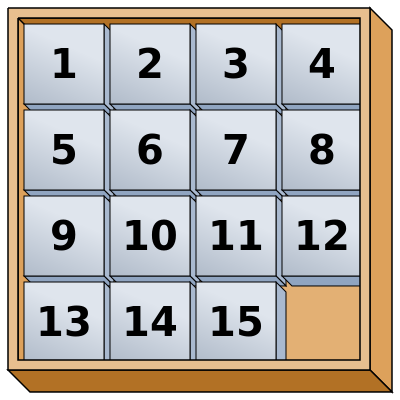
\includegraphics[width=0.3\textwidth]{solved.png}
\centering
\caption{A Solved Board}
\end{figure}

\item \textbf{Valid State:} Any state generated by the successor() is valid, where each tiles occupies exactly one place.

\item \textbf{State Space: } State Space is the collection of all the states that have been discovered but not visited, they are stored in a fringe, which constantly pops the state with the lowest cost (i.e. the sum of g(s) +
f(s)).

\item \textbf{Successor Functions: } Through each state there are 4 possible states, wherein the tile can slide D, U, R, L into the empty place. Technically only 3 would be good to use depending upon the previous state, otherwise you would be replicating the parent state by moving back in the same position. Eg: If your parent is L, then moving in the Right direction would lead you back to the same state, hence we can eliminate that.

\item \textbf{Cost Functions: } Cost Function is the cost of travelling from one state to another which is 1 for each movement. Also we use a heuristic to estimate the length of the goal which helps us get to the solution quicker than the brute force way.
\end{itemize}

\textbf{Implementation Details:}
Try to make your solver as fast as possible. Which heuristic functions did you try, and which works
best?
\begin{itemize}
\item We tried three different heuristics:
\begin{itemize}
\item \textbf{Hamming Distance: } This heuristic calculates the number of misplaced tiles. In other words, all it does is that it checks whether if a tile is in its location, if not adds 1 to the cost. This is \textbf{not} a particularly good estimate of how far are we from the solution. The idea of a heuristic is to estimate the distance from the goal which in turn allows us to select a good probable path. Even though this is admissible since it does not overestimate the cost, it duly underestimates it most of the times.
\item \textbf{Permutation Inversion: } This heuristic particularly checks for inversion, which means it checks how many pairs are out of order. This is often times \textbf{not admissible} and hence can be discarded, since heuristic functions do not allow us to overestimate the distance to the goal.
\item \textbf{Manhattan Distance: } This heuristic calculates the steps for each tile to reach its correct position when no other tiles is on the table. This is the \textbf{best of the three}, since it does not over estimate but also gives us a fair amount of idea as to how far are we from the solution.
\end{itemize} 
\item We implemented A\* search algorithm to find the optimal path to the solution, code would be present in the \textit{problem2} folder.

\item Tests carried for professors input, we obtain a path of 24 steps (LLUURULULDRDRDRRULDRUUUL) within about 2 seconds (0:00:02.189130) on our local machines. There are various test cases we tried, some take a while and some happen quickly, it fairly depends upon the complexity of the input.
\end{itemize}
\end{homeworkProblem}

\clearpage

%----------------------------------------------------------------------------------------
%	PROBLEM 3
%----------------------------------------------------------------------------------------

% To have just one problem per page, simply put a \clearpage after each problem

\begin{homeworkProblem}
\textbf{The Marriage Problem Abstraction: }
\begin{itemize}
\item \textbf{Monte Carlo Descent}
\begin{itemize}
\item \textbf{State Space: } Represented by an M-element vector, where the index of each element corresponds to a certain guest, and each element has a non-negative integer as its value corresponding to the index of the table where the guest are seated. M is the total number of the guests.

\item \textbf{Initial State: } No guests have been seated in any table, represented by an m-element vector where each element is set to 0, which means that the corresponding guest has not been seated in any table yet.

\item \textbf{Goal State: } Every guest has been seated in a table and the number of the tables is as least as possible, represented by an m-element vector where no elements are 0 and the maximum element is as least as possible.

\item \textbf{Cost Function: } It equals to the number of the tables.

\item \textbf{Successor function: } Assign a table to a guest who has not been seated yet, given the condition that 
\begin{enumerate}
\item This new state is never visited before
\item After assigning, the number of guests in the assigned table will not exceed a given number N, and
\item Guests in that table do not know each other before.
item It is represented by assigning a positive integer P to an element which is currently 0, and making sure that after assigning
\begin{itemize}
\item The new state is not in our visited state records.
\item The number of P in the vector will not exceed N.
\item Guests with the index that has an element of P do not know each other.
\end{itemize}
\end{enumerate}

\item \textbf{Edge Weights: } It will equal 0 or 1. If after assigning, there will be one more table, then edge weight equals to 1. Otherwise, if the number of tables do not change, the edge weight equals to 0.

\item \textbf{Heuristic Function: } It equals to the number of the tables,. Since we directly take the cost function as the heuristic function, it must be admissible.
\begin{gather*}
h(s) = number of tables
\end{gather*}

\item \textbf{Algorithm:}
\begin{itemize}
\item Repeat L times (in my code, L = 10 * the number of the guests):
\item s = initial state
\item Repeat K times (in my code, K = 10 * the number of the guests):
\begin{itemize}
\item If s is our goal, then return s
\item Pick s\textsc{\char13} from the successors of s at random
\item If h(s\textsc{\char13}) $\leq$ h(s) (we want to find the s\textsc{\char13} that makes h(s\textsc{\char13}) as least as possible!), then s = s\textsc{\char13}
\item Else with probability of exp(-(h(s\textsc{\char13})-h(s))/T), s = s\textsc{\char13}
In my code, because h(s\textsc{\char13}) is either equal to h(s) or 1 $\geq$ h(s), so in this case I can directly replace $h(s\textsc{\char13})-h(s)$ by 1. And $T = MAX_TEMPERATURE *(1 – the times we repeat 2)/K)$, which makes T decrease as the times we repeat 2) increases.

\item After repeating Step 1 and 2 L times, L results will be got. Then the algorithm compares the results with each other based on the number of the tables and chooses the result with the least number of tables as the final result.
\end{itemize}
\item The problem I met is though Monte Carlo is much faster, it struggles to get the best result sometimes when just running it once. Therefore I repeat it several times and choose the best result as the final result.
\end{itemize}
\end{itemize}

\item \textbf{A\* Search}
The Abstract is similar to Monte Carlo
\begin{itemize}
\item \textbf{State Space: } Represented by an M-element vector, where the index of each element corresponds to a certain guest, and each element has a non-negative integer as its value corresponding to the index of the table where the guest are seated. M is the total number of the guests.
\item \textbf{Initial State: } No guests have been seated in any table, represented by an m-element vector where each element is set to 0, which means that the corresponding guest has not been seated in any table yet.
\item \textbf{Goal State: } Every guest has been seated in a table and the number of the tables is as least as possible, represented by an m-element vector where no elements are 0 and the maximum element is as least as possible.
\item \textbf{Cost Function :} It equals to the number of the tables.
\item \textbf{Successor Function: } Assign a table to a guest who has not been seated yet, given the condition that 1) this new state is never visited before, 2) after assigning, the number of guests in the assigned table will not exceed a given number N, and 3) guests in that table do not know each other before. It is represented by assigning a positive integer P to an element which is currently 0, and making sure that after assigning, 1) the new state is not in our visited state records, 2) the number of P in the vector will not exceed N, and 3) guests with the index that has an element of P do not know each other.

\item \textbf{Edge Weights: } It will equal 0 or 1. If after assigning, there will be one more table, then edge weight equals to 1. Otherwise, if the number of tables do not change, the edge weight equals to 0.

\item \textbf{Heuristic Function: } t equals to the number of the tables,. Since we directly take the cost function as the heuristic function, it must be admissible.
\begin{gather*}
h(s) = number of tables
\end{gather*}

\item \textbf{Algorithm: }
\begin{itemize}
\item Add initial state to the fringe. The fringe is implemented by using a priority queue (in Python, it’s called heapq). The priority is generated first based on the number of the tables in the state. If there are two states with the same total number of the tables, then they will be compared based on the order they are added to the fringe.
\item Repeated while fringe is not empty:
\begin{itemize}
\item Pop the head h of the fringe
\item If h is our goal, return h
\item Push the successors of h into the fringe
\end{itemize}
\item Return False

\end{itemize}
\end{itemize}
\end{itemize}
\end{homeworkProblem}



\clearpage

%----------------------------------------------------------------------------------------
%	REFERENCES
%----------------------------------------------------------------------------------------

\begin{homeworkProblem}[References]
\begin{enumerate}
\item \href{https://en.wikipedia.org/wiki/15_puzzle#/media/File:15-puzzle.svg}{15 Puzzle solved image}
\item \href{http://mathworld.wolfram.com/PermutationInversion.html}{Wolfram}
\item \href{http://www.jaapsch.net/puzzles/javascript/fifteenj.htm}{Puzzle Generator}
\item \href{http://www.geeksforgeeks.org/check-instance-15-puzzle-solvable/}{Solvability Test}
\item \href{https://www.cs.princeton.edu/courses/archive/fall12/cos226/assignments/8puzzle.html}{Solvability}
\item \href{http://codereview.stackexchange.com/questions/33473/solving-15-puzzle}{Stack Exchange}
\item \href{http://codegolf.stackexchange.com/questions/6884/solve-the-15-puzzle-the-tile-sliding-puzzle}{Stack Exchange}
\end{enumerate}
\clearpage
\end{homeworkProblem}

%----------------------------------------------------------------------------------------

\end{document}